
\section{Results}
\label{sec:results}

\subsection{Campaign Validity}
\label{sec:validity}

All $12{,}960$ runs of the main campaign completed. Completion is 1.0000 in
every run, minimum and mean alike, and the total teleport count is zero, so no
run was discarded and no context was excluded: all 648 are analysed, each with
four policies at five seeds. The campaign contains approximately 22.0 million
simulated vehicle trips. Because validity is exact rather than near-exact, none
of the results below involves a selection decision about which runs to keep.

\subsection{Policy Complementarity}
\label{sec:complementarity}

\paragraph{The confirmatory gate}
Gate G1$'$, declared before the campaign and evaluated on all 648 contexts,
\textbf{passes}: three policies --- P1, P3 and P4 --- are strictly best in at
least one context with a resolved margin, against the threshold of three. The
resolved winner counts are P3 227, P4 19 and P1 11, with 257 of 648 contexts
resolved. \textbf{P2 is never a resolved winner}, which confirms on the full
factor space what the screen saw in its 16 contexts. The screen's STOP verdict
was therefore a sampling artefact of the screening design rather than a property
of the portfolio: the screen had the power to detect near-ties, which it did
correctly, but not the coverage to find the regions where P1 and P4 win.

\paragraph{Ties are common and are reported as such}
In 50 of 648 contexts (7.7\,\%) two or more policies produce exactly equal system
mean journey time, because at low demand or low penetration they route the guided
cohort identically. The tied sets are P2 with P4 in 39 contexts, P2 with P3 and
P4 in 8, and P3 with P4 in 3. Under the declared tie-break the winner counts are
P3 418, P4 129, P2 80 and P1 21; restricting to the 598 contexts with a unique
minimum gives P3 415, P4 129, P2 33 and P1 21. We report both, because a count
that changes by 47 contexts depending on how ties are broken should not be
presented as a single number.

\paragraph{Most differences do not survive replication}
Of the 648 contexts, 391 (60.3\,\%) have an unresolved winning margin. Those
margins are negligible rather than merely uncertain: their median is 0.13\,\% of
the best journey time, against a median of 5.20\,\% among resolved margins, which
reach 26.9\,\% (Fig.~\ref{fig:comp}b). With five paired seeds under common random
numbers a 5\,\% difference resolves comfortably, so the unresolved cases are
genuine equivalence and not a power failure. The portfolio is complementary, but
in most contexts the choice among its members does not matter on journey time.

\paragraph{Two policies are largely interchangeable}
Applying the study's operational-identity criterion --- an unresolved paired
difference together with a route split differing by less than 2\,\% of the guided
cohort --- P2 and P4 are indistinguishable in 42.6\,\% of contexts, P2 and P3 in
22.7\,\%, and P3 and P4 in 20.2\,\%. P1 is never indistinguishable from any other
policy, which is expected: it is the only policy that ignores traffic state.
Averaged over the six pairs the identity rate is 14.2\,\%. A nominal portfolio of
four policies therefore behaves, over much of the context space, like a portfolio
of two or three.

\paragraph{The winner map is multi-factor but shallow}
Fig.~\ref{fig:comp}a shows the modal winner over the demand-by-penetration
plane. Predicting the winner with a constant is correct in 64.5\,\% of contexts;
the best single factor, demand, reaches 66.5\,\%; the best pair, demand with
penetration, reaches 70.7\,\%; the best triple, demand with green ratio and
penetration, reaches 79.2\,\%; and all six factors together identify the winner
in every context by construction. The structure is genuinely multi-factor --- no
single factor comes close --- but it is also shallow, in the sense that the
marginal return to context information falls off quickly after the first two
factors. This is the first indication that the decision problem, although real,
is not large.

\begin{table}[htbp]
\centering\scriptsize
\caption{Complementarity of the portfolio over 648 contexts on the primary
criterion, and over all three criteria jointly. ``Best'' uses the declared
portfolio-order tie-break; ``unique best'' counts only the 598 contexts with a
unique minimum; ``resolved best'' requires the margin over the runner-up to
exceed twice its paired standard error.}
\label{tab:comp}
\setlength{\tabcolsep}{3.4pt}
\begin{tabular}{@{}lrrrrr@{}}
\toprule
& P1 & P2 & P3 & P4 & total\\
\midrule
Best on journey time & 21 & 80 & 418 & 129 & 648\\
\quad of which unique best & 21 & 33 & 415 & 129 & 598\\
\quad of which resolved best & 11 & \textbf{0} & 227 & 19 & 257\\
Best on \CO & 10 & 57 & 453 & 128 & 648\\
Best on stopped delay & 0 & 80 & 139 & \textbf{429} & 648\\
In the three-criterion Pareto set & 21 & 266 & 555 & 525 & ---\\
\midrule
\multicolumn{6}{@{}l}{\emph{Operationally indistinguishable pairs} (share of 648 contexts)}\\
\multicolumn{6}{@{}l}{\quad P2--P4 42.6\,\%; \ P2--P3 22.7\,\%; \ P3--P4 20.2\,\%; \ P1 with any other 0.0\,\%}\\
\midrule
\multicolumn{6}{@{}l}{\emph{Winner-map classification rate}}\\
\multicolumn{6}{@{}l}{\quad constant 64.5\,\%; \ best single (demand) 66.5\,\%; \ best pair (demand, penetr.) 70.7\,\%}\\
\multicolumn{6}{@{}l}{\quad best triple (demand, green, penetr.) 79.2\,\%; \ all six factors 100\,\%}\\
\bottomrule
\end{tabular}
\end{table}

\begin{figure}[htbp]
\centering
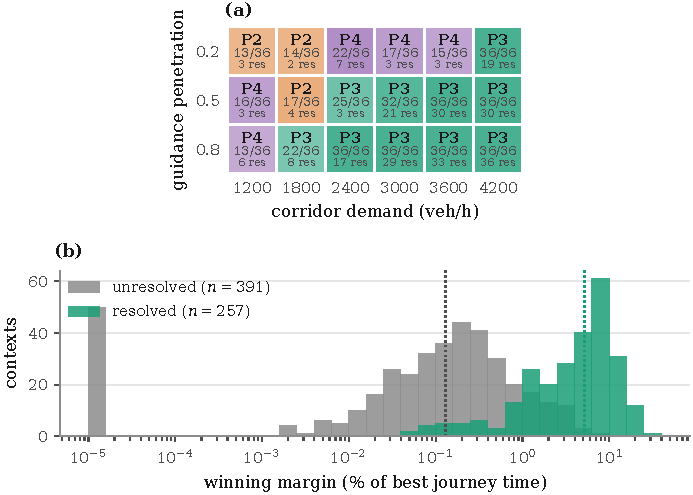
\includegraphics[width=\linewidth]{figures/fig2_complementarity.pdf}
\caption{(a) Modal winning policy over the demand-by-penetration plane, each
cell aggregating 36 contexts; the fraction is the modal winner's share of those
contexts and ``res'' counts contexts whose winning margin is resolved against
replication noise. (b) Distribution of the winning margin, as a percentage of the
best journey time in that context, separated into resolved and unresolved
contexts. Dotted lines mark the two medians. The axis is logarithmic and exact
ties are shown at the left edge.}
\label{fig:comp}
\end{figure}

\subsection{Mechanisms and Preference Boundaries}
\label{sec:mechanism}

The winner map has a physical reading. Fig.~\ref{fig:cost} shows why the
portfolio separates at all: the distance-minimising policy P1 diverges from the
other three as demand rises, because it concentrates the guided cohort on the
arterial regardless of whether the arterial can carry it, while the three
traffic-aware policies remain within a few per cent of each other throughout.
The same figure shows the penetration effect that Section~\ref{sec:lit:routing}
would predict: mean journey time under the traffic-aware policies falls from
penetration 0.2 to 0.5 and then rises again at 0.8, while P1 deteriorates
monotonically. More guidance is not monotonically better, consistent with
\citet{yang1998penetration} and with the concentration mechanism reported by
\citet{cornacchia2026concentration}, although this study does not isolate that
mechanism and the agreement is a consistency check rather than a replication.

\begin{figure}[htbp]
\centering
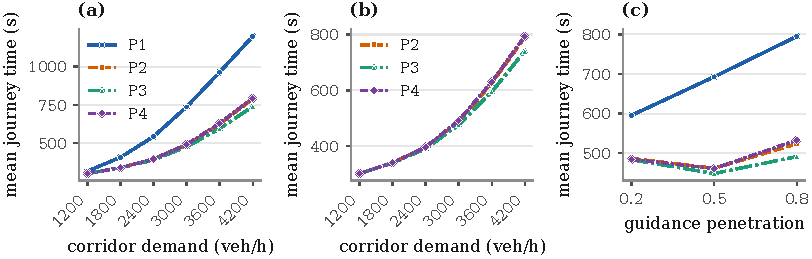
\includegraphics[width=\linewidth]{figures/fig3_cost_landscape.pdf}
\caption{System mean journey time against (a, b) corridor demand and (c)
guidance penetration, averaged over all other factors. Panel (b) repeats panel
(a) without P1 so that the three traffic-aware policies can be distinguished.
Colours and markers are consistent across panels.}
\label{fig:cost}
\end{figure}

Fitting the depth-2 mechanistic rule to the winner's identity on all 648
contexts, for exposition, gives a first split on $x_8 = pD/\mathrm{cap}_C$, the
share of the shortest corridor's capacity that the guided cohort alone would
consume, at a threshold bracketed between the adjacent sampled values 0.748 and
0.781. Below that threshold the rule separates on the effective green ratio;
above it, on whether total demand exceeds arterial capacity. Fig.~\ref{fig:mech}
shows the corresponding structure directly: below $x_8 \approx 0.76$ the
reliability-aware and reactive policies win a substantial share of contexts, and
above it the load-balancing policy wins almost everywhere.

The reading is that the controlling quantity is not demand and not penetration
separately but their product relative to the capacity of the corridor that every
policy would otherwise prefer. When the guided cohort alone would saturate the
arterial, spreading it across corridors is worth doing; when it would not,
spreading it costs more than it saves. That is a statement about association
within a designed factorial. The experiment varies the factors but does not
isolate the mechanism --- it contains no treatment that changes $x_8$ while
holding the physical routes constant --- so no causal claim is made, and the rule
is reported as consistent with the data rather than as identified by it.

\begin{figure}[htbp]
\centering
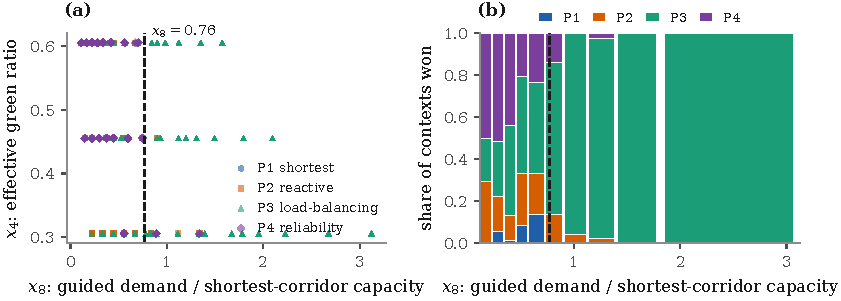
\includegraphics[width=\linewidth]{figures/fig4_mechanism.pdf}
\caption{(a) Contexts in the plane of controlled-flow saturation $x_8$ and
effective green ratio $x_4$, coloured by the winning policy; the dashed line is
the first split of the depth-2 rule fitted to all contexts. (b) Share of
contexts won by each policy in deciles of $x_8$. The transition is a property of
$x_8$ rather than of demand or penetration separately.}
\label{fig:mech}
\end{figure}

\paragraph{Refining the boundary}
Nineteen demand transitions were refined from a 600\,veh/h grid to a 150\,veh/h
grid. Thirteen of them have a single changepoint on the refined grid, and for
nine of those the point-estimate bracket narrows to 150\,veh/h; the remaining
four stay at 600. The other six transitions are \emph{not} monotone in demand:
the winner changes two to five times across the refined sequence. Moreover, of
the thirteen single-changepoint transitions, only seven have either endpoint of
the changepoint interval resolved against replication noise. The honest summary
is that refinement narrows a point estimate but does not deliver a resolved
boundary: a grid cannot locate a boundary more finely than its own spacing, and
at this spacing the winner sequence is, in a third of cases, not even monotone.
No continuous threshold is reported anywhere in this paper.

\subsection{Decision Value}
\label{sec:value}

This is the central result. The single best fixed policy over all 648 contexts is
P3, with a system mean journey time of 474.35\,s per vehicle. The hindsight best
achieves 473.90\,s. The decision headroom is therefore
\begin{equation}
H = 474.35 - 473.90 = 0.45\ \text{s per vehicle},
\end{equation}
which is 0.095\,\% of the fixed policy's own mean cost. Averaging the per-context
ratio instead gives 0.120\,\%; the two are different statistics and the
aggregate is used throughout, with its denominator stated.

Against that, the cost of choosing the wrong fixed policy is large.
Table~\ref{tab:value} gives the penalties: committing to P1 for the whole
benchmark costs 220.21\,s per vehicle more than committing to P3, which is
46.4\,\% of P3's mean cost. P2 and P4 cost 16.34\,s (3.4\,\%) and 18.34\,s
(3.9\,\%). The ratio between the first-order decision --- which fixed policy ---
and the second-order decision --- whether to adapt it --- is roughly 490 to 1.
Fig.~\ref{fig:value}a places the two on the same axis, which requires a
logarithmic scale.

\begin{table}[htbp]
\centering\small
\caption{Decision value on the primary criterion over 648 contexts. Penalty is
the mean cost above the single best fixed policy; headroom is the mean cost of
the single best fixed policy above the per-context best.}
\label{tab:value}
\begin{tabular}{@{}lrrr@{}}
\toprule
Choice & Mean journey & Penalty & Penalty\\
 & time (s/veh) & (s/veh) & (\%)\\
\midrule
Fix P1 (shortest) & 694.56 & 220.21 & 46.42\\
Fix P4 (reliability) & 492.69 & 18.34 & 3.87\\
Fix P2 (reactive) & 490.69 & 16.34 & 3.44\\
Fix P3 (load balancing, SBS) & 474.35 & 0.00 & ---\\
\midrule
Hindsight best (VBS) & 473.90 & $-0.45$ & $-0.095$\\
\bottomrule
\end{tabular}
\end{table}

\paragraph{Why the headroom is so small}
The fixed policy is near-dominant rather than merely good. P3 attains the
per-context minimum in 426 of 648 contexts (65.7\,\%). In the 222 contexts where
it does not, it loses on average 1.32\,s and at worst 17.19\,s. In the contexts
where it does win, it wins by 22.47\,s on average. The upside of the fixed policy
is therefore about 17 times its downside, and an adaptive layer competes only
for the downside. A portfolio can be complementary in the sense of
Section~\ref{sec:complementarity} while this ratio makes adaptation nearly
worthless, and that is what happens here.

\paragraph{Most of the headroom is not resolvable}
The headroom must also be compared against the replication noise of the
experiment that measured it. Fig.~\ref{fig:value}c plots, for each of the 222
contexts where the fixed policy is not best, the headroom in that context against
that context's own $2\,$SE band on the paired difference. Only 55 of the 222
(24.8\,\%) carry a headroom larger than their own noise band. The mean noise band
in those contexts is 1.67\,s, against a mean headroom of 1.32\,s. Resolving the
campaign-wide mean effect of 0.45\,s at the same criterion would require
approximately 25 seeds per context rather than five, that is about 64{,}800 runs
instead of 12{,}960. This is stated as a property of the effect size, not as a
recommendation: an effect that needs 25 replications per cell to separate from
simulation noise is unlikely to be the deciding consideration in a deployment.

\begin{figure}[htbp]
\centering
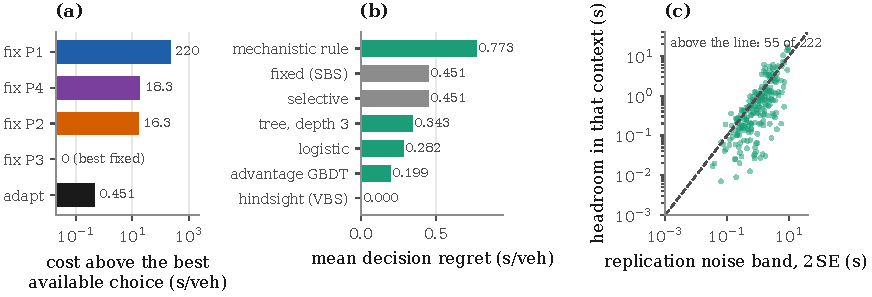
\includegraphics[width=\linewidth]{figures/fig5_decision_value.pdf}
\caption{(a) Cost of each available commitment above the best one, on a
logarithmic axis: the penalty for the wrong fixed policy dwarfs the headroom
available to adaptation. (b) Mean decision regret of every rule under
leave-one-context-out evaluation. (c) For each of the 222 contexts where the
fixed policy is not the per-context best, the headroom in that context against
its own replication noise band; points above the dashed line are contexts whose
headroom exceeds the dispersion of the experiment that measured it.}
\label{fig:value}
\end{figure}
